
\documentclass[a4paper,12pt]{scrbook}
\usepackage{amsmath,amssymb,amsthm}
\usepackage{fancyvrb}
\usepackage{parskip}
\usepackage{lastpage}
\usepackage{verbatim,boxedminipage,enumitem}
\usepackage{ifthen}
\usepackage{color,graphicx}
\usepackage{pgf}
\usepackage{longtable}
\usepackage{upquote}
%\usepackage[all]{xy}
\usepackage{tobiShell}
\usepackage{tikz}
\usetikzlibrary{automata}
\usetikzlibrary{arrows}
\usepackage{pgf,pgfarrows,pgfnodes}
\usepackage{pgfplots}
\usepackage{circuitikz}
\usetikzlibrary{circuits}
\usetikzlibrary{circuits.logic.US}
\usepackage{mymath}
\usepackage{python}
%------------------------------------------------------------------
% Verbatim for console window - single line frame, no line numbers
%------------------------------------------------------------------
\DefineVerbatimEnvironment%
 {console}{Verbatim}
 {frame=single}

%--------------------------------------------------------
% Remove the vertical spacing before and after Verbatim.
%--------------------------------------------------------
\usepackage{atbeginend}
\BeforeBegin{console}{\mbox{}\\ \begin{minipage}{\textwidth}\vspace{3pt}}
\AfterEnd{console}{\vspace{4pt} \end{minipage} \\ }

\begin{document}
\thispagestyle{empty}

\begin{center}
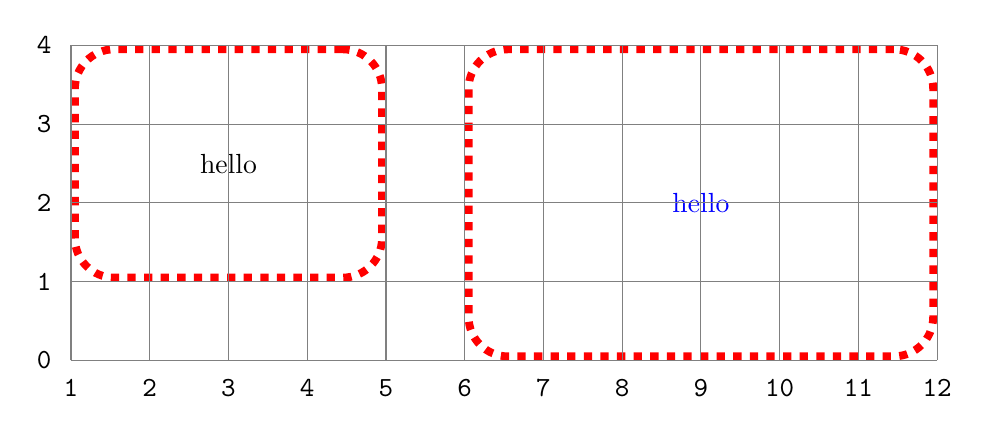
\begin{tikzpicture}

\draw (3.0, 2.5)
  node[draw, line width=0.1cm, dashed, color=red,
       rounded corners=0.5cm, inner sep=0cm] {

\begin{minipage}[t][2.9cm]{3.9cm}
\mbox{}

\end{minipage}

};\draw (3.0, 2.5) node[color=black] {hello};
\draw (9.0, 2.0)
  node[draw, line width=0.1cm, dashed, color=red,
       rounded corners=0.5cm, inner sep=0cm] {

\begin{minipage}[t][3.9cm]{5.9cm}
\mbox{}

\end{minipage}

};\draw (9.0, 2.0) node[color=blue] {hello};\draw[gray] (1.0,0.0) -- (1.0,4);
\draw[gray] (2.0,0.0) -- (2.0,4);
\draw[gray] (3.0,0.0) -- (3.0,4);
\draw[gray] (4.0,0.0) -- (4.0,4);
\draw[gray] (5.0,0.0) -- (5.0,4);
\draw[gray] (6.0,0.0) -- (6.0,4);
\draw[gray] (7.0,0.0) -- (7.0,4);
\draw[gray] (8.0,0.0) -- (8.0,4);
\draw[gray] (9.0,0.0) -- (9.0,4);
\draw[gray] (10.0,0.0) -- (10.0,4);
\draw[gray] (11.0,0.0) -- (11.0,4);
\draw[gray] (12.0,0.0) -- (12.0,4);
\draw[gray] (1.0,0.0) -- (12,0.0);
\draw[gray] (1.0,1.0) -- (12,1.0);
\draw[gray] (1.0,2.0) -- (12,2.0);
\draw[gray] (1.0,3.0) -- (12,3.0);
\draw[gray] (1.0,4.0) -- (12,4.0);
\draw(1, 0) node [font=\ttfamily, label=below:{\texttt{1}}] {};
\draw(2, 0) node [font=\ttfamily, label=below:{\texttt{2}}] {};
\draw(3, 0) node [font=\ttfamily, label=below:{\texttt{3}}] {};
\draw(4, 0) node [font=\ttfamily, label=below:{\texttt{4}}] {};
\draw(5, 0) node [font=\ttfamily, label=below:{\texttt{5}}] {};
\draw(6, 0) node [font=\ttfamily, label=below:{\texttt{6}}] {};
\draw(7, 0) node [font=\ttfamily, label=below:{\texttt{7}}] {};
\draw(8, 0) node [font=\ttfamily, label=below:{\texttt{8}}] {};
\draw(9, 0) node [font=\ttfamily, label=below:{\texttt{9}}] {};
\draw(10, 0) node [font=\ttfamily, label=below:{\texttt{10}}] {};
\draw(11, 0) node [font=\ttfamily, label=below:{\texttt{11}}] {};
\draw(12, 0) node [font=\ttfamily, label=below:{\texttt{12}}] {};
\draw(1, 0) node [font=\ttfamily, label=left:{\texttt{0}}] {};
\draw(1, 1) node [font=\ttfamily, label=left:{\texttt{1}}] {};
\draw(1, 2) node [font=\ttfamily, label=left:{\texttt{2}}] {};
\draw(1, 3) node [font=\ttfamily, label=left:{\texttt{3}}] {};
\draw(1, 4) node [font=\ttfamily, label=left:{\texttt{4}}] {};
\end{tikzpicture}

\end{center}

\end{document}
